\section{Ejercicio 3}
\subsection*{A)}
Para terminar de pintar la pantalla creamos una funci\'on en screen.c, iniciarPantalla. El pseudoc\'odigo de la misma es el siguiente:
\begin{codesnippet}
\begin{verbatim}
void iniciar_pantalla()
{	
	clockd[0] = '|';
	clockd[1] = '/';
	clockd[2] = '-';
	clockd[3] = '\\';
	Debugger = 0;
	
	unsigned int x,y;
	const char* texto = " ";
	//Los espacios en negro:
	for (x = 0; x < 80; x++)
	{
			print(texto, x, 0, 0x00);
			print(texto, x, 45, 0x00);
			print(texto, x, 46, 0x00);
			print(texto, x, 47, 0x00);
			print(texto, x, 48, 0x00);
			print(texto, x, 49, 0x00);	
	} 
	
	for (x = 35; x < 45; x++)
	{
		for (y = 45; y < 50; y++)
		{
			if (x < 40)
			{
				print(texto, x, y, 0x44);	//Franja roja (4 = rojo)
			}
			else
			{
				print(texto, x, y, 0x11);	//Franja azul (1 = azul)
			}
		}	
	}
\end{verbatim}
\end{codesnippet}
\begin{codesnippet}
\begin{verbatim}
	texto = "1 2 3 4 5 6 7 8";
	print(texto, 5, 46, 0x0f);
	print(texto, 60, 46, 0x0f);
	print("( )", 75, 49, 0x0f);
	texto = "# # # # # # # #";	//relojes
	print(texto, 5, 48, 0x0f);
	print(texto, 60, 48, 0x0f);

	print("G", 0, 1, 0x44);
	print("G", 79, 1, 0x11);
	
	puntaje_o_restantes(juego.puntaje_B , 41, 47, 0x1f);
	puntaje_o_restantes(juego._20A, 31, 47, 0x4f);
	puntaje_o_restantes(juego.puntaje_A , 36, 47, 0x4f);
	puntaje_o_restantes(juego._20B, 49, 47, 0x1f);
	
}
\end{verbatim}
\end{codesnippet}

\subsection*{B)}

El procesador posee una unidad de manejo de memoria, MMU, (Memory Management Unit) que es un dispositivo de Hardware responsable del manejo de los accesos a memorias, entre 
algunas de sus funciones. Este dispositivo se va a encargar  de la traducci\'on de las direcciones l\'ogicas (o virtuales) a direcciones f\'isicas (o reales) que enviara por el 
bus de address hacia la memoria externa. Para representar esto se cuenta  con un directorio de paginas, cada pagina tiene un tamaño de 4k y 1024 descriptores de 8 bytes. Cada uno 
representa en los bits 31 a 12  el valor correspondiente a la direcci\'on f\'isica de la Pagina (el Page Frame) que contiene la tabla de descriptores de pagina, cada una de estas 
con 1024 descriptores. Adem\'as  cada descriptor de 32 bits posee las siguientes caracter\'isticas:\newline

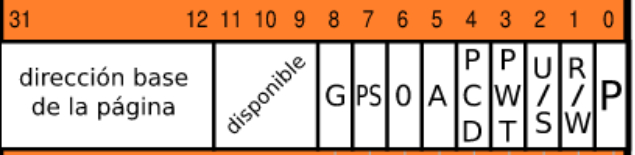
\includegraphics[width=\textwidth,height=1.0in,keepaspectratio
]{imagen.jpg}\newline

Para representar los descriptores y con esto el directorio de paginas se utilizo un str en lenguaje C, como el que se muestra a continuaci\'on y en el archivo mmu.c		\newline
\begin{codesnippet}
\begin{verbatim}
typedef struct str_mmu_entry{ 
	\textit{	unsigned char p:1;
		unsigned char rw:1; 
		unsigned char us:1; 
		unsigned char pwt:1;
		unsigned char pcd:1; 
		unsigned char a:1; 
		unsigned char ign:1;
		unsigned char ps:1; 
		unsigned char g:1;
		unsigned char disp:3; 
		unsigned int  base\_0\_20  :20; }
} \textit{__attribute__((__packed__, aligned (4))) mmu_entry};
\end{verbatim}
\end{codesnippet}
estructura que representa un descriptor de directorio de pagina y de la page table. Si bien entre si difieren algunos de sus par\'ametros, los que lo hacen no se utilizan.\newline \newline

\subsubsection*{mmu\_inicializar\_dir\_kernel()}
En la page table  cada descriptor, con el atributo P=1, contiene la direcci\'on de una pagina  correspondiente  a una Tabla de Paginas. Este es el ultimo nivel de traducci\'on. Cada pagina es de 4K, con 1024 descriptores de 4bytes cada uno. Y cada uno de estos posee en los  bits 31 a 12,  el Page Frame de la pagina de memoria, es decir los 20 bits mas significativos de la direcci\'on f\'isica de memoria en donde comienza la pagina.\newline
Como se desea crear un directorio de paginas que mapee usando identity mapping, las direcciones 0x00000000 a 0x3FFFFF, se necesita completar 1 pagina, de la page table  ya que cada descriptor se corresponde con un pagina en direcci\'on f\'isica de 4K y en total se estar\'ian completando  1024 descriptores, como cada uno se corresponde con 4k obtenemos 1024*4  = 0x400000 que es  lo que necesitamos direccionar.  Como fue necesaria una pagina,  se completó un  descriptor de la page directory  con los siguientes atributos (la inicializaci\'on de todos las paginas y descriptores mencionados se encuentran mmu.c). En primer lugar se declaro que la direcci\'on inicial del directorio de pagina es la 0x27000: \textit{ mmu\_entry *pd = ( mmu\_entry *) 0x27000; p = 1; rw = 1; us = 0; pwt = 0; pcd = 0; a = 0;  ign = 0; ps = 0; g = 0; disp = 0;} debido a que los 20 bits mas significativos constituyen la  direcci\'on del directorio de pagina, se shiftea 12 bits hacia la izquierda para quedarnos con los restantes $base\_0\_20$ = (0x28000 + i*0x1000) $>>$ 12;  \newline
Como cada pagina posee 1024 descriptores, el resto de los descriptores sin usar fueron inicializados con los mismo atributos excepto que P=0 , ya que no se necesitan.
Una vez realizado esto se inicializaron los ya mencionados descriptores de pagina.  Como ya se cuenta con un directorio de pagina inicializado en la direcci\'on 0x27000 y esta ocupa 0x1000, las tablas de pagina van a comenzar a partir de la direcci\'on 0x28000. Y los atributos tendr\'an el valor \textit{mmu\_entry *pt = (mmu\_entry *) 0x28000 ; p = 1; rw = 1; us = 0; pwt = 0; pcd = 0; a = 0; ign = 0; ps = 0; g = 0; disp = 0; base\_page\_0\_20 = i*0x1000}; Donde 0 $<=$ i $<=$ 1024, ya que de esta manera se direcciona a los primero 4Mb de memoria.\newline \newline

\subsection*{C)}
En $kernel.asm$ llamamos a mmu\_inicializar lo que hace es empezar un contador de páginas libres. Llamamos a mmu\_inicializar\_dir\_kernel que hace lo descripto arriba. \newline
Colocamos en CR3 0x27000 porque es donde empieza la page directory y seteamos el primer bit de CR0, todo esto para habilitar paginación. 


\subsection*{D)}
Creamos un texto con el nombre del grupo de la misma forma que estaba hecho para \newline$Iniciando kernel (Modo Real)...$(en $kernel.asm$), luego utilizando imprimir\_texto\_mp, 
imprimimos el texto que definimos. Para centrarlo a derecha a 80 le restamos la longitud del texto y este valor lo pusimos en $y$, 
como tiene que estar en la primera fila $x$ es 0. El color que elegimos fue gris con fondo negro por eso pusimos 0x07 para el color.
